\documentclass[journal]{IEEEtran}
%
\usepackage{instructivo}  % Commands for multiple choice
\usepackage{float}
\graphicspath{{./}{./fig/}}

\usepackage[natbib=true,style=trad-unsrt,backend=biber]{biblatex}

\addbibresource{literatura.bib}

% correct bad hyphenation here
\hyphenation{op-tical net-works semi-conduc-tor}


\begin{document}
%
% paper title
% Titles are generally capitalized except for words such as a, an, and, as,
% at, but, by, for, in, nor, of, on, or, the, to and up, which are usually
% not capitalized unless they are the first or last word of the title.
% Linebreaks \\ can be used within to get better formatting as desired.
% Do not put math or special symbols in the title.
\title{Experimento 8: Respuesta en frecuencia de un amplificador}


\author{~ Sebastián Calvo Fong ~,~\IEEEmembership{Estudiante,~ITCR}
        y ~ Juan Esteban Obando Pérez ~,~\IEEEmembership{Estudiante,~ITCR,}
}


% The paper headers
\markboth{EL3215 Laboratorio de Electrónica Analógica, IS2026}%
{EL3215 Laboratorio de Electrónica Analógica}


% make the title area
\maketitle


\begin{abstract}
En esta práctica se analizó el comportamiento de un amplificador bipolar en configuración de emisor común, evaluando su desempeño tanto en frecuencias bajas como altas. Se llevaron a cabo cálculos teóricos, simulaciones y mediciones reales para examinar los parámetros de polarización en corriente continua, el comportamiento en corriente alterna y la respuesta espectral del circuito. En la primera fase se determinó la ganancia de tensión y se comprobó la polarización adecuada del transistor, encontrándose una buena correspondencia entre los valores predichos, los simulados y los medidos experimentalmente. En una segunda etapa se incorporaron capacitores adicionales que modelan las capacitancias internas del dispositivo, con el fin de observar cómo afectan la ganancia y la frecuencia de corte superior. Los resultados obtenidos confirmaron la validez de las técnicas de análisis empleadas y evidenciaron el efecto de las capacitancias parásitas en la reducción de la respuesta del amplificador cuando la frecuencia de la señal se eleva.
\end{abstract}

% Se sugiere no más de cuatro palabras o frases cortas en orden alfabético, separadas por comas, que representen su reporte
\begin{IEEEkeywords}
Amplificador, frecuencia, capacitancia, corriente, voltaje.
\end{IEEEkeywords}


%%%%%%%%%%%%%%%%%%%%%%%%%%%%%%%%%%%%%%%%%%%%%%%%%%%%%%%%%%%%%%%%%%%%%%%%%%%%%%%%%%%%%%%%%%%%%%
%%%%%%%%%%%%%%%%%%%%%%%%%%%%%%%%%%%%%%%%%%%%%%%%%%%%%%%%%%%%%%%%%%%%%%%%%%%%%%%%%%%%%%%%%%%%%%
\section{Introducción}

\IEEEPARstart{E}{n} electrónica, el análisis de la respuesta en frecuencia de un amplificador permite describir cómo varía su ganancia en función de la frecuencia de la señal de entrada. En los amplificadores con transistores bipolares de unión (BJT), este comportamiento está determinado principalmente por los condensadores de acoplamiento, los condensadores de desvío y las capacitancias internas del propio transistor. A bajas frecuencias, la reactancia de los condensadores aumenta, limitando el paso de la señal y reduciendo la ganancia; mientras que a altas frecuencias, el efecto Miller junto con las capacitancias internas provocan también una disminución de la respuesta.

El estudio de la respuesta en frecuencia permite determinar las frecuencias críticas inferior y superior, que definen el rango de operación efectivo del amplificador. En este experimento se analizó un amplificador BJT de una etapa para caracterizar su comportamiento tanto en bajas como en altas frecuencias, empleando modelos equivalentes RC simplificados y verificando los resultados mediante mediciones experimentales.

El objetivo general fue analizar la respuesta en frecuencia de un amplificador en emisor común, determinando sus frecuencias de corte inferior y superior mediante cálculos y mediciones. Con ello se buscó comprender la influencia de los elementos capacitivos y de las características internas del transistor sobre el desempeño del circuito, un aspecto fundamental en el diseño de amplificadores electrónicos [Floyd2008].


%%%%%%%%%%%%%%%%%%%%%%%%%%%%%%%%%%%%%%%%%%%%%%%%%%%%%%%%%%%%%%%%%%%%%%%%%%%%%%%%%%%%%%%%%%%%%%
%%%%%%%%%%%%%%%%%%%%%%%%%%%%%%%%%%%%%%%%%%%%%%%%%%%%%%%%%%%%%%%%%%%%%%%%%%%%%%%%%%%%%%%%%%%%%%
\section{Respuesta Del Amplificador En Baja Frecuencia}

La respuesta en baja frecuencia de un amplificador BJT de una etapa está gobernada por los condensadores de acoplamiento y de desvío, los cuales determinan el comportamiento del circuito cuando la frecuencia de la señal de entrada disminuye. Estos condensadores permiten el paso de la señal de corriente alterna mientras bloquean los niveles de corriente continua, asegurando la adecuada polarización del transistor y el acoplamiento entre etapas. A medida que la frecuencia de entrada se reduce, la reactancia capacitiva de estos elementos aumenta, limitando la transferencia de señal y produciendo una disminución de la ganancia.

\begin{equation}
X_C = \frac{1}{2\pi f C}
\end{equation}

Este fenómeno produce una atenuación progresiva del nivel de salida conforme la señal se aproxima hacia e límite inferior de la banda de paso. Cada condensador, desde el de entrada hasta el de salida, introduce una frecuencia crítica de corte inferior distinta. La respuesta global del amplificador en bajas frecuencias está dominada por aquel condensador cuya frecuencia de corte sea mayor, ya que determina el punto donde la ganancia comienza a decrecer. La suma de los efectos de todos los condensadores define la frecuencia crítica mínima inferior, la cual establece el inicio de la región de atenuación.
Comprender el comportamiento se vuelve crucial en las etapas de diseño y ajuste de los amplificadores, ya que el valor de los condensadores de acoplamiento debe seleccionarse de modo que el circuito mantenga una ganancia constante en el rango de las frecuencias de interés. La adecuada elección de los componentes es esencial para evitar distorsiones por pérdida de señal en frecuencias bajas y preservar la fidelidad [Floyd2008]. El análisis de respuestas individuales permite modelar el circuito en equivalentes RC que ayudan a la simplificación de la respuesta en conjunto.

\begin{figure}[H]
\centering
\begin{subfigure}[c]{0.4\textwidth}
	\centering
	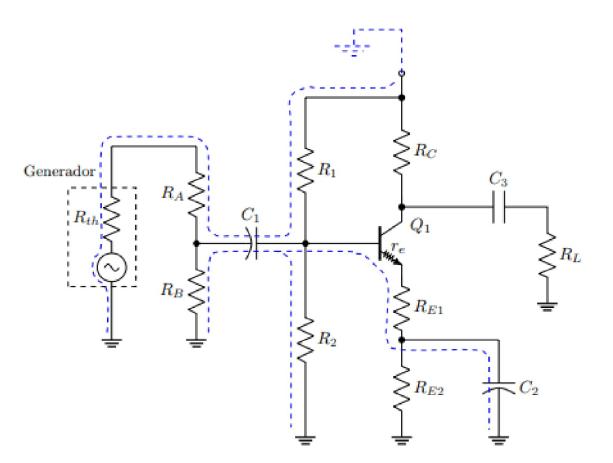
\includegraphics[width=2.5in]{fig/figura1.PNG}
	\label{fig:directa}	
\end{subfigure}
\hfill
\caption{Amplificador Emisor Comun: Rutas de carga y descarga}
\label{fig:Amplificador B1}
\end{figure}

%%%%%%%%%%%%%%%%%%%%%%%%%%%%%%%%%%%%%%%%%%%%%%%%%%%%%%%%%%%%%%%%%%%%%%%%%%%%%%%%%%%%
%%%%%%%%%%%%%%%%%%%%%%%%%%%%%%%%%%%%%%%%%%%%%%%%%%%%%%%%%%%%%%%%%%%%%%%%%%%%%%%%%%%%
\subsection{Circuitos de Medición}

El circuito de la Fig. \ref{fig:Amplificador B2}   consiste en un amplificador de una sola etapa en configuración de emisor común, utilizando un transistor BJT 2N3904. La polarización se establece mediante un divisor de tensión formado por $R_1$ ($68\text{ k}\Omega$) y $R_2$ ($10\text{ k}\Omega$), con una fuente de alimentación $V_{CC}$ de $15\text{ V}$. Para estabilizar la ganancia y el punto de operación, se emplea una resistencia de emisor dividida ($R_{E1}$ y $R_{E2}$). El diseño integra condensadores de acoplamiento en la entrada ($C_1$) y salida ($C_2$) para bloquear la componente de CD de la señal, además de un condensador de derivación ($C_3$) en paralelo con $R_{E2}$ para maximizar la ganancia de corriente alterna en la banda media.

\begin{figure}[H]
\centering
\begin{subfigure}[c]{0.4\textwidth}
	\centering
	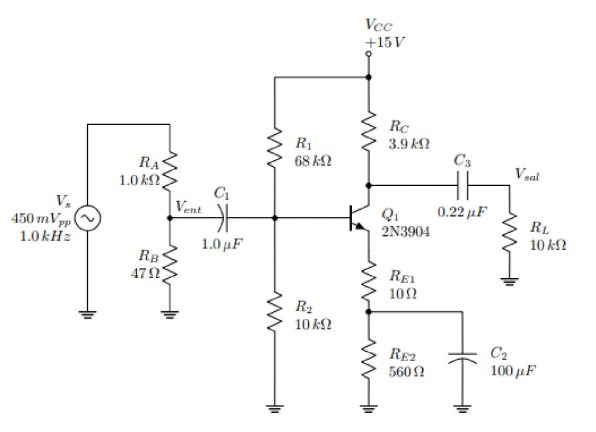
\includegraphics[width=2.5in]{fig/figura2.PNG}
	\label{fig:directa}	
\end{subfigure}
\hfill
\caption{Amplificador Emisor Comun}
\label{fig:Amplificador B2}
\end{figure}

%%%%%%%%%%%%%%%%%%%%%%%%%%%%%%%%%%%%%%%%%%%%%%%%%%%%%%%%%%%%%%%%%%%%%%%%%%%%%%%%%%%%
%%%%%%%%%%%%%%%%%%%%%%%%%%%%%%%%%%%%%%%%%%%%%%%%%%%%%%%%%%%%%%%%%%%%%%%%%%%%%%%%%%%%
\subsection{Instrumentos de medición necesarios}
\begin{itemize}
  \item1 resistencia de 10 $\Omega$
	\item 1 resistencia de 47 $\Omega$
	\item 1 resistencia de 560 $\Omega$
	\item 1 resistencia de 1.0 $\text{ k}\Omega$
	\item 1 resistencia de 3.9 $\text{ k}\Omega$
	\item 2 resistencias de 10 $\text{ k}\Omega$
	\item 1 resistencia de 68 $\text{ k}\Omega$
	\item 1 capacitor de 0.22 $\mu F$
	\item 1 capacitor de 1.0 $\mu F$
	\item 1 capacitor de 100 $\mu F$
	\item 2 capacitores de 1000 $\mu F$
	\item 1 transistor 2N3904 NPN
\end{itemize}

%%%%%%%%%%%%%%%%%%%%%%%%%%%%%%%%%%%%%%%%%%%%%%%%%%%%%%%%%%%%%%%%%%%%%%%%%%%%%%%%%%%%
%%%%%%%%%%%%%%%%%%%%%%%%%%%%%%%%%%%%%%%%%%%%%%%%%%%%%%%%%%%%%%%%%%%%%%%%%%%%%%%%%%%%
\subsection{Simulaciones}

Antes de realizar las mediciones experimentales en el laboratorio, se efectuaron simulaciones del circuito amplificador utilizando los valores nominales de los componentes indicados en el procedimiento. El propósito de estas simulaciones fue observar de forma preliminar la respuesta en baja frecuencia del amplificador y estimar los puntos de operación de corriente y tensión, así como las variaciones en la ganancia para diferentes frecuencias de entrada. 

Se realizó el montaje de un circuito con configuración de emisor común que permitió analizar la baja frecuencia aplicando técnicas de análisis para elementos activos. Los cálculos teóricos de los parámetros en corriente continua y corriente alterna se llevaron a cabo utilizando superposición de fuentes, ley de Ohm y las expresiones matemáticas establecidas en el instructivo.

A partir de los resultados obtenidos, se registraron los valores simulados correspondientes a los parámetros del transistor — $V_B$, $V_E$, $V_C$ e $I_E$— además de las frecuencias de corte asociadas a los condensadores $C_1$, $C_2$ y $C_3$. Estos datos sirvieron como referencia para comparar posteriormente con las mediciones experimentales. Los resultados de estas simulaciones de baja frecuencia se detallan en la Tabla \ref{tab:simulacion_baja}, donde se contrastan con los valores calculados teóricamente.

\begin{table}[!htbp]
\centering
\caption{Simulaciones del amplificador en emisor común: Parámetros CD y CA}
\begin{tabular}{|c|c|c|}
\hline
\textbf{Parámetro} & \textbf{Valor calculado} & \textbf{Valor simulado} \\
\hline
$V_B$ & 1.82 V & 1.92 V \\
\hline
$V_E$ & 1.12 V & 1.22 V \\
\hline
$I_E$ & 1.97 mA & 1.64 mA \\
\hline
$V_C$ & 7.31 V & 6.6 V \\
\hline
$V_{CE}$ & 6.19 V & 5.38 V \\
\hline
$r_e'$ & 13.19 $\Omega$ & 11.7 $\Omega$ \\
\hline
$A_v$ & -120 & -130 \\
\hline
$V_{out}$ & 2.13 Vpp & 2.5 Vpp \\
\hline
\end{tabular}
\label{tab:simulacion_baja}
\end{table}

\begin{table}[H]
\centering
\caption{Simulaciones del amplificador en emisor común: Resistencias equivalentes para cada capacitor de acople}
\begin{tabular}{|c|c|}
\hline
\textbf{Capacitor} & $\mathbf{R_{eq}}$ \\
\hline
$C_1$ & 3.38 k$\Omega$ \\
\hline
$C_2$ & 26 k$\Omega$ \\
\hline
$C_3$ & 14 k$\Omega$ \\
\hline
\end{tabular}
\label{tab:req_baja}
\end{table}

\begin{table}[H]
\centering
\caption{Simulaciones del amplificador en emisor común: Frecuencias críticas de corte inferior}
\begin{tabular}{|c|c|}
\hline
\textbf{Capacitor} & $\mathbf{f_{critica}}$ \\
\hline
$C_1$ & 47 Hz \\
\hline
$C_2$ & 61 Hz \\
\hline
$C_3$ & 52 Hz \\
\hline
\textbf{General} & \textbf{160 Hz} \\
\hline
\end{tabular}
\label{tab:frecuencias_baja}
\end{table}


%%%%%%%%%%%%%%%%%%%%%%%%%%%%%%%%%%%%%%%%%%%%%%%%%%%%%%%%%%%%%%%%%%%%%%%%%%%%%%%%%%%%
%%%%%%%%%%%%%%%%%%%%%%%%%%%%%%%%%%%%%%%%%%%%%%%%%%%%%%%%%%%%%%%%%%%%%%%%%%%%%%%%%%%%
\subsection{Resultados experimentales}

En la primera fase del experimento, se obtuvieron los valores para polarización en corriente continua del transistor 2N3904, los cuales se detallan en la Tabla \ref{tab:experimento_baja}. Los resultados experimentales muestran un punto de operación estable, con un voltaje colector-emisor ($V_{CE}$) medido de $6.02\text{ V}$ y una corriente de emisor ($I_E$) de $1.94\text{ mA}$, lo que confirma que el dispositivo se encuentra operando dentro de la región activa para garantizar una amplificación lineal.  

Respecto al análisis de corriente alterna en la banda media, se registró una ganancia de tensión ($A_v$) de $-115$, valor que muestra una concordancia satisfactoria con el parámetro calculado de $-120$. Un valor negativo en la ganancia de un amplificador indica que la señal de salida está invertida 180 grados respecto a la entrada. 

\begin{table}[!ht]
\centering
\caption{Valores de resistencias utilizadas}
\begin{tabular}{|c|c|c|}
\hline
\textbf{Resistor} & \textbf{Valor requerido} & \textbf{Valor medido} \\
\hline
$R_A$ & 1 k$\Omega$ & 998.19 $\Omega$ \\
\hline
$R_B$ & 47 $\Omega$ & 46.19 $\Omega$ \\
\hline
$R_1$ & 68 k$\Omega$ & 66.56 k$\Omega$ \\
\hline
$R_2$ & 10 k$\Omega$ & 9.84 k$\Omega$ \\
\hline
$R_{E1}$ & 10 $\Omega$ & 10.06 $\Omega$ \\
\hline
$R_{E2}$ & 560 $\Omega$ & 550.04 $\Omega$ \\
\hline
$R_C$ & 3.9 k$\Omega$ & 3.84 k$\Omega$ \\
\hline
$R_L$ & 10 k$\Omega$ & 9.86 k$\Omega$ \\
\hline
\end{tabular}
\label{tab:resistencias}
\end{table}

\begin{table}[!ht]
\centering
\caption{Amplificador en emisor común: Parámetros CD y CA}
\begin{tabular}{|c|c|c|}
\hline
\textbf{Parámetro} & \textbf{Valor calculado} & \textbf{Valor medido} \\
\hline
$V_B$ & 1.82 V & 1.84 V \\
\hline
$V_E$ & 1.12 V & 1.15 V \\
\hline
$I_E$ & 1.97 mA & 1.94 mA \\
\hline
$V_C$ & 7.31 V & 7.17 V \\
\hline
$V_{CE}$ & 6.19 V & 6.02 V \\
\hline
$r_e'$ & 13.19 $\Omega$ & 12 $\Omega$ \\
\hline
$A_v$ & -120 & -115 \\
\hline
$V_{out}$ & 2.13 Vpp & 2.3 Vpp \\
\hline
\end{tabular}
\label{tab:experimento_baja}
\end{table}

En cuanto a la respuesta en baja frecuencia, se determinaron las frecuencias críticas individuales asociadas a los condensadores de acoplamiento y de derivación, según se muestra en la Tabla \ref{tab:req2_baja}. La frecuencia de corte inferior general medida fue de $200\text{ Hz}$, lo que representa una desviación moderada respecto a los $160\text{ Hz}$ obtenidos teóricamente, atribuible a las tolerancias de los componentes capacitivos utilizados.

\begin{table}[!ht]
\centering
\caption{Amplificador en emisor común: Resistencias equivalentes para cada capacitor de acople}
\begin{tabular}{|c|c|}
\hline
\textbf{Capacitor} & $\mathbf{R_{eq}}$ \\
\hline
$C_1$ & 3.15 k$\Omega$ \\
\hline
$C_2$ & 22.30 k$\Omega$ \\
\hline
$C_3$ & 13.85 k$\Omega$ \\
\hline
\end{tabular}
\label{tab:req2_baja}
\end{table}

\begin{table}[!ht]
\centering
\caption{Amplificador en emisor común: Frecuencias críticas de corte inferior}
\begin{tabular}{|c|c|}
\hline
\textbf{Capacitor} & $\mathbf{f_{critica}}$ \\
\hline
$C_1$ & 52 Hz \\
\hline
$C_2$ & 72.6 Hz \\
\hline
$C_3$ & 53 Hz \\
\hline
\textbf{General} & \textbf{200 Hz} \\
\hline
\end{tabular}
\label{tab:frecuencias2_baja}
\end{table}


%%%%%%%%%%%%%%%%%%%%%%%%%%%%%%%%%%%%%%%%%%%%%%%%%%%%%%%%%%%%%%%%%%%%%%%%%%%%%%%%%%%%
%%%%%%%%%%%%%%%%%%%%%%%%%%%%%%%%%%%%%%%%%%%%%%%%%%%%%%%%%%%%%%%%%%%%%%%%%%%%%%%%%%%%
\subsection{Análisis de resultados}

La estabilidad del punto de operación es un parámetro importante para el comportamiento espectral del amplificador. Los valores medidos en el laboratorio ($V_B = 1.84\text{ V}$ y $V_{CE} = 6.02\text{ V}$) presentan concordancia con los valores teóricos calculados ($V_B = 1.82\text{ V}$ y $V_{CE} = 6.19\text{ V}$), lo que ratifica el diseño del divisor de tensión y la estabilidad que ofrece la resistencia de emisor. Esta correcta polarización asegura que el transistor opere en la región activa, permitiendo una excursión de señal simétrica en la banda media de frecuencias.

En el régimen de baja frecuencia, la ganancia de tensión medida fue de $-115$, mostrando una ligera reducción respecto al valor calculado de $-120$. La configuración de emisor común mostró el signo negativo durante los cálculos y al visualizar la onda, lo cual representa el desfase de 180 grados característico de esta configuración. La frecuencia de corte inferior general medida ($f_L$) se situó en $200\text{ Hz}$, frente a los $160\text{ Hz}$ proyectados teóricamente. Esta discrepancia del $25\%$ se explica mediante el análisis de las redes RC individuales. El polo dominante fue introducido por el capacitor de salida $C_2$, con una frecuencia medida de $72.6\text{ Hz}$. La diferencia entre los valores teóricos y prácticos en esta zona se atribuye principalmente a las tolerancias de los capacitores electrolíticos ($10\%$-$20\%$), los cuales alteran las constantes de tiempo $\tau = RC$ y desplazan el límite inferior de la banda pasante hacia frecuencias más elevadas.

%%%%%%%%%%%%%%%%%%%%%%%%%%%%%%%%%%%%%%%%%%%%%%%%%%%%%%%%%%%%%%%%%%%%%%%%%%%%%%%%%%%%
%%%%%%%%%%%%%%%%%%%%%%%%%%%%%%%%%%%%%%%%%%%%%%%%%%%%%%%%%%%%%%%%%%%%%%%%%%%%%%%%%%%%
\section{Respuesta Del Amplificador En Baja Frecuencia}

A frecuencias elevadas, el comportamiento del amplificador de emisor común deja de ser constante y comienza a presentar una atenuación en la ganancia de tensión. El fenómeno es provocado principalmente por las capacitancias internas del transistor, específicamente la capacitancia de unión base-emisor ($C_{be}$) y la capacitancia base-colector ($C_{bc}$). A medida que la frecuencia de la señal de entrada aumenta, la reactancia de estos elementos disminuye, creando trayectorias de derivación para la señal que reducen progresivamente la amplitud de la salida [Boylestad2009].  

El factor determinante en este régimen de operación es el efecto Miller, el cual afecta a la red de entrada en una configuración inversora. Debido a la ganancia de tensión inversa del amplificador, la capacitancia $C_{bc}$ se refleja en la entrada multiplicada por un factor de $(1 + |A_{v}|)$, generando una capacitancia de entrada efectiva ($C_{ent}$) significativamente mayor a los valores parásitos nominales. Este incremento en la capacitancia total de entrada reduce la frecuencia de corte superior ($f_{cu}$), limitando el ancho de banda efectivo del amplificador y su capacidad para procesar señales de alta velocidad sin pérdida de integridad [Floyd2008].  

El análisis en alta frecuencia es necesario para entender las limitaciones físicas que tiene el dispositivo y cómo las impedancias de la fuente y de carga interactúan con las redes capacitivas. En el desarrollo del experimento, el fenómeno se analiza mediante la adición de capacitores externos que funcionan como una simulación del comportamiento de las capacitancias internas del transistor en una escala de frecuencia medible para el laboratorio. Este procedimiento permite validar los modelos teóricos de polos y ceros, que facilita la comprensión de la respuesta dinámica y la estabilidad del sistema frente a variaciones en la frecuencia de la señal. 

%%%%%%%%%%%%%%%%%%%%%%%%%%%%%%%%%%%%%%%%%%%%%%%%%%%%%%%%%%%%%%%%%%%%%%%%%%%%%%%%%%%%
%%%%%%%%%%%%%%%%%%%%%%%%%%%%%%%%%%%%%%%%%%%%%%%%%%%%%%%%%%%%%%%%%%%%%%%%%%%%%%%%%%%%
\subsection{Circuitos de Medición}

En esta fase de la Fig. \ref{fig:Amplificador B3} se utiliza la misma topología de emisor común, pero se modifica el esquema para modelar el comportamiento del amplificador ante frecuencias elevadas. Para ello, se incorporan condensadores externos adicionales que simulan las capacitancias internas parásitas del transistor, específicamente la capacitancia base-emisor ($C_{be}$) y la capacitancia base-colector ($C_{bc}$). Esta configuración permite observar de forma experimental el efecto Miller, donde la capacitancia base-colector se ve multiplicada por la ganancia del circuito, creando un polo de baja frecuencia en la entrada que limita el ancho de banda superior y reduce la ganancia conforme aumenta la frecuencia de operación.

\begin{figure}[H]
\centering
\begin{subfigure}[c]{0.4\textwidth}
	\centering
	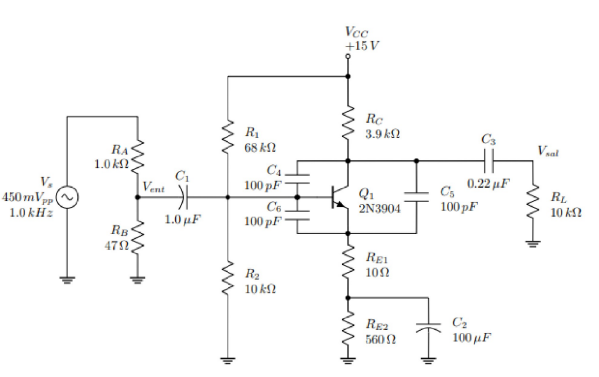
\includegraphics[width=2.5in]{fig/figura4.PNG}
	\label{fig:directa}	
\end{subfigure}
\hfill
\caption{Amplificador en emisor común para pruebas en alta frecuencia}
\label{fig:Amplificador B3}
\end{figure}

\subsection{Instrumentos de medición necesarios}
\begin{itemize}
  \item1 Mismos componentes y circuito
	\item 3 capacitores de 100 $\unit{pF}$ adicionales
\end{itemize}


%%%%%%%%%%%%%%%%%%%%%%%%%%%%%%%%%%%%%%%%%%%%%%%%%%%%%%%%%%%%%%%%%%%%%%%%%%%%%%%%%%%%
%%%%%%%%%%%%%%%%%%%%%%%%%%%%%%%%%%%%%%%%%%%%%%%%%%%%%%%%%%%%%%%%%%%%%%%%%%%%%%%%%%%%
\subsection{Simulaciones}

En la segunda fase, la simulación se trasladó hacia un enfoque de la respuesta ante señales de alta frecuencia. Para ello, se integraron en el esquema de anterior condensadores externos destinados a modelar las capacitancias internas parásitas del transistor BJT, específicamente las asociadas a las uniones base-emisor y base-colector. 

Así mismo, se determinó de manera preliminar la frecuencia de corte superior ($f_H$) y se analizó la pendiente de atenuación del circuito al operar fuera de la banda media. El modelado de estos componentes internos fue fundamental para establecer el ancho de banda total del sistema.  El circuito de medición puede representarse también mediante su modelo de análisis de alta frecuencia de la Fig. \ref{fig:Amplificador B4}.

\begin{figure}[H]
\centering
\begin{subfigure}[c]{0.4\textwidth}
	\centering
	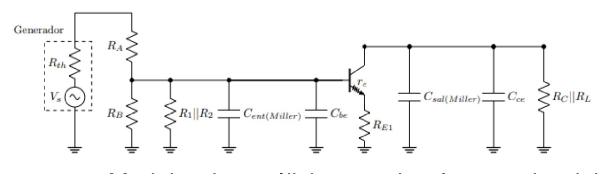
\includegraphics[width=2.5in]{fig/figura3.PNG}
	\label{fig:directa}	
\end{subfigure}
\hfill
\caption{Modelo de análisis en alta frecuencia del amplificador en emisor común}
\label{fig:Amplificador B4}
\end{figure}

Finalmente, se registraron los valores de ganancia y desfase obtenidos en esta etapa espectral, los cuales sirvieron como punto de comparación para evaluar las discrepancias introducidas por elementos no ideales del montaje real. Los resultados de estas simulaciones de alta frecuencia se detallan en la Tabla \ref{tab:simulacion_alta}, donde se contrastan con los valores calculados teóricamente.

\begin{table}[H]
\centering
\caption{Simulación de parámetros CD y CA del emisor común para pruebas en alta frecuencia}
\begin{tabular}{|c|c|c|}
\hline
\textbf{Parámetro} & \textbf{Valor calculado} & \textbf{Valor simulado} \\
\hline
$V_B$ & 1.84 V & 1.814 V \\
\hline
$V_E$ & 1.14 V & 1.162 V \\
\hline
$I_E$ & 1.99 mA & 2 mA \\
\hline
$V_C$ & 7.23 V & 7.088 V \\
\hline
$V_{CE}$ & 6.09 V & 5.929 V \\
\hline
$r_e'$ & 13.07 $\Omega$ & 13 $\Omega$ \\
\hline
$A_v$ & -121.8 & -115.08 \\
\hline
$V_{out}$ & 2.46 Vpp & 2.29 Vpp \\
\hline
\end{tabular}
\label{tab:simulacion_alta}
\end{table}

\begin{table}[H]
\centering
\caption{Mediciones de la simulación para respuesta en alta frecuencia}
\begin{tabular}{|c|c|}
\hline
\textbf{Parámetro} & \textbf{Valor calculado} \\
\hline
$C_{ent}$ & 12.38 $\unit{nF}$ \\
\hline
$R_{eq}$ & 44.24 $\Omega$ \\
\hline
$f_{Cent}$ & 290.6 kHz \\
\hline
$C_{sal}$ & 200.82 $\unit{pF}$ \\
\hline
$R_{CE}$ & 2.81 $\text{ k}\Omega$ \\
\hline
$f_{Csal}$ & 282.2 kHz \\
\hline
\end{tabular}
\label{tab:simulacion2_alta}
\end{table}

\begin{table}[H]
\centering
\caption{Valor simulado de la frecuencia crítica superior general}
\begin{tabular}{|c|c|c|}
\hline
\textbf{Parámetro} & \textbf{Valor calculado} & \textbf{Valor simulado} \\
\hline
$f_{CU}$ & 143.3 kHz & 170 kHz \\
\hline
\end{tabular}
\label{tab:simulacion3_alta}
\end{table}


%%%%%%%%%%%%%%%%%%%%%%%%%%%%%%%%%%%%%%%%%%%%%%%%%%%%%%%%%%%%%%%%%%%%%%%%%%%%%%%%%%%%
%%%%%%%%%%%%%%%%%%%%%%%%%%%%%%%%%%%%%%%%%%%%%%%%%%%%%%%%%%%%%%%%%%%%%%%%%%%%%%%%%%%%
\subsection{Resultados experimentales}

En la fase experimental de alta frecuencia, se verificaron primero los parámetros de polarización descritos en la Tabla \ref{tab:exp_alta}. Se obtuvo un voltaje de base ($V_B$) de 1.83 V y un voltaje colector-emisor ($V_{CE}$) de 6.02 V, valores que aseguran la operación en la región activa del transistor. La ganancia de tensión medida en la banda media fue de -112.5, con un voltaje de salida de 2.25 Vpp. Al incrementar la frecuencia de la señal, se determinó experimentalmente una frecuencia de corte superior ($f_{CU}$) de 140 kHz, lo cual muestra una alta correlación con el valor calculado de 143.3 kHz.

De igual manera, se caracterizaron las redes capacitivas del montaje físico, con una capacitancia de entrada ($C_{ent}$) de 11.45 nF y una frecuencia crítica de entrada ($f_{C\_ent}$) de 313.56 kHz. Por su parte, la red de salida presentó una capacitancia ($C_{sal}$) de 200.89 pF y una frecuencia crítica ($f_{C\_sal}$) de 286.67 kHz. La proximidad entre los valores medidos de la Tabla \ref{tab:exp2_alta} y los simulados confirma la validez de los modelos de pequeña señal empleados para describir el comportamiento del amplificador en el límite superior de su ancho de banda.

\begin{table}[H]
\centering
\caption{Parámetros CD y CA del emisor común para pruebas en alta frecuencia}
\begin{tabular}{|c|c|c|}
\hline
\textbf{Parámetro} & \textbf{Valor calculado} & \textbf{Valor medido} \\
\hline
$V_B$ & 1.84 V & 1.837 V \\
\hline
$V_E$ & 1.14 V & 1.152 V \\
\hline
$I_E$ & 1.99 mA & 2 mA \\
\hline
$V_C$ & 7.23 V & 7.170 V \\
\hline
$V_{CE}$ & 6.09 V & 6.022 V \\
\hline
$r_e'$ & 13.01 $\Omega$ & 13 $\Omega$ \\
\hline
$A_v$ & -121.8 & -112.5 \\
\hline
$V_{out}$ & 2.46 Vpp & 2.25 Vpp \\
\hline
\end{tabular}
\label{tab:exp_alta}
\end{table}

\begin{table}[H]
\centering
\caption{Mediciones para respuesta en alta frecuencia}
\begin{tabular}{|c|c|}
\hline
\textbf{Parámetro} & \textbf{Valor obtenido} \\
\hline
$C_{ent}$ & 11.45 $\unit{nF}$ \\
\hline
$R_{eq}$ & 44.33 $\Omega$ \\
\hline
$f_{Cent}$ & 313.56 kHz \\
\hline
$C_{sal}$ & 200.89 $\unit{pF}$ \\
\hline
$R_{CE}$ & 2.76 $\text{ k}\Omega$ \\
\hline
$f_{Csal}$ & 282.67 kHz \\
\hline
\end{tabular}
\label{tab:exp2_alta}
\end{table}

\begin{table}[H]
\centering
\caption{Valor simulado de la frecuencia crítica superior general}
\begin{tabular}{|c|c|c|}
\hline
\textbf{Parámetro} & \textbf{Valor calculado} & \textbf{Valor medido} \\
\hline
$f_{CU}$ & 143.3 kHz & 140 kHz \\
\hline
\end{tabular}
\label{tab:exp3_alta}
\end{table}


%%%%%%%%%%%%%%%%%%%%%%%%%%%%%%%%%%%%%%%%%%%%%%%%%%%%%%%%%%%%%%%%%%%%%%%%%%%%%%%%%%%%
%%%%%%%%%%%%%%%%%%%%%%%%%%%%%%%%%%%%%%%%%%%%%%%%%%%%%%%%%%%%%%%%%%%%%%%%%%%%%%%%%%%%
\subsection{Análisis de resultados}

A frecuencias elevadas, el comportamiento del circuito dejó de ser independiente de la frecuencia debido a la reactancia de las capacitancias internas emuladas del transistor ($C_{be}$ y $C_{bc}$). El fenómeno más crítico observado fue el Efecto Miller, que multiplicó la capacitancia base-colector por el factor de ganancia ($1 + |A_v|$), resultando en una capacitancia de entrada efectiva ($C_{ent}$) de $11.45\text{ nF}$. Esta capacitancia, en conjunto con la resistencia equivalente de la fuente ($R_{eq} = 44.33\text{ }\Omega$), formó un filtro pasa-bajas que limitó drásticamente el ancho de banda superior. 

Se obtuvo una frecuencia de corte superior medida de $140\text{ kHz}$, la cual es extremadamente cercana al valor teórico calculado de $143.3\text{ kHz}$. Sin embargo, existe una desviación notable respecto al valor simulado de $170\text{ kHz}$. Esta diferencia sugiere que el modelo del componente en Multisim subestima las capacitancias parásitas reales del transistor 2N3904 o no contabiliza las capacitancias inherentes del montaje en físico, las cuales suelen añadir trayectorias de derivación adicionales para la señal. 

La caída de ganancia registrada en esta etapa confirma que el amplificador cumple con el comportamiento de un sistema de primer orden en alta frecuencia, donde el ancho de banda se ve restringido por las limitaciones físicas del dispositivo semiconductor. 


%%%%%%%%%%%%%%%%%%%%%%%%%%%%%%%%%%%%%%%%%%%%%%%%%%%%%%%%%%%%%%%%%%%%%%%%%%%%%%%%%%%%
%%%%%%%%%%%%%%%%%%%%%%%%%%%%%%%%%%%%%%%%%%%%%%%%%%%%%%%%%%%%%%%%%%%%%%%%%%%%%%%%%%%%
\section{Conclusiones}

En conclusión, se validó la estabilidad del punto de operación en corriente continua del transistor 2N3904, logrando voltajes de polarización ($V_B = 1.84\text{ V}$ y $V_{CE} = 6.02\text{ V}$) acordes a los calculados teóricamente. Esto asegura el correcto funcionamiento del transistor en su configuración de amplificador de emisor común. La condición garantiza que el dispositivo operara en la región activa, que permite la amplificación lineal con una ganancia de tensión en la banda media de $-115$ y un desfase característico de un emisor común de $180^\circ$. 

El comportamiento en baja frecuencia está determinado por las redes RC de acoplamiento y derivación, donde el capacitor de salida $C_2$ se identificó como el polo dominante al presentar la frecuencia crítica medida más elevada ($72.6\text{ Hz}$). La discrepancia del $25\%$ observada en la frecuencia de corte inferior general respecto a la teoría ($200\text{ Hz}$ frente a $160\text{ Hz}$) se atribuye a las tolerancias intrínsecas en los capacitores electrolíticos del laboratorio, que alteran las constantes de tiempo. 

Se comprobó que el límite superior de operación del amplificador está restringido por las capacitancias internas del semiconductor y la influencia del efecto Miller. El fenómeno incrementó la capacitancia de entrada efectiva a $11.45\text{ nF}$, reduciendo la frecuencia de corte superior ($f_{CU}$) a $140\text{ kHz}$. La cercanía del resultado con el valor teórico de $143.3\text{ kHz}$ valida la precisión de los modelos de pequeña señal para predecir el ancho de banda del circuito. 

La comparación entre dominios reveló que, si bien la teoría y la práctica presentan una alta coincidencia, las simulaciones computacionales pueden sobreestimar el desempeño del amplificador por los modelos de transistores idealizados, que subestiman las capacitancias parásitas del montaje físico o cuentan con parámetros diferentes a los físicos. 

En este experimento, la influencia de la protoboard y el cableado contribuyó a una atenuación más temprana de la señal en comparación con el entorno simulado. Para obtener simulaciones más fidedignas a la realidad es necesario ajustar los parámetros internos del transistor computacional para que se ajuste aún más al modelo físico.

Finalmente, se cumplió el objetivo de caracterizar la respuesta espectral del amplificador en emisor común, determinando un ancho de banda efectivo comprendido entre los $200\text{ Hz}$ y los $140\text{ kHz}$. Este análisis permitió cuantificar las limitaciones físicas del dispositivo y comprender cómo la selección de componentes capacitivos define el rango de operación útil en aplicaciones de audio y procesamiento de señales. 

%%%%%%%%%%%%%%%%%%%%%%%%%%%%%%%%%%%%%%%%%%%%%%%%%%%%%%%%%%%%%%%%%%%%%%%%%%%%%%%%%%%%
%%%%%%%%%%%%%%%%%%%%%%%%%%%%%%%%%%%%%%%%%%%%%%%%%%%%%%%%%%%%%%%%%%%%%%%%%%%%%%%%%%%%

\begin{thebibliography}{1}

\bibitem{Floyd2008}
T. L. Floyd, \emph{Dispositivos electrónicos}, 8va ed. México: Pearson Educación, 2008.

\bibitem{Boylestad2009}
R. L. Boylestad y L. Nashelsky, \emph{Electrónica: Teoría de Circuitos y Dispositivos Electrónicos}, 10ma ed. México: Pearson Educación, 2009.

\bibitem{ITCR2026}
S. Calvo y J. Obando, ``Experimento 8: Respuesta en frecuencia de un amplificador,'' Guía de Laboratorio EL3215, Tecnológico de Costa Rica, I Semestre, 2026.

\end{thebibliography}


%%%%%%%%%%%%%%%%%%%%%%%%%%%%%%%%%%%%%%%%%%%%%%%%%%%%%%%%%%%%%%%%%%%%%%%%%%%%%%%%%%%%
%%%%%%%%%%%%%%%%%%%%%%%%%%%%%%%%%%%%%%%%%%%%%%%%%%%%%%%%%%%%%%%%%%%%%%%%%%%%%%%%%%%%
\begin{IEEEbiographynophoto}{Sebastián Calvo-Fong}
Estudiante de ingeniería en electrónica del Tecnológico de Costa Rica. 
Correo: s.calvo.1@estudiantec.cr
\end{IEEEbiographynophoto}

\begin{IEEEbiographynophoto}{Juan Esteban Obando-Pérez}
Estudiante de ingeniería en electrónica del Tecnológico de Costa Rica. 
Correo: j.obando.1@estudiantec.cr
\end{IEEEbiographynophoto}

\vfill

\end{document}






